% general distance smoothing stuff

\label{chap-gds}


\section{Introduction}

The previous chapter makes clear that there are two conflicting issues impeding the utility of this approach to smoothing over complex regions. The first is that the ordering of the points in space must be maintained, but (second) once a sufficiently high dimensional projection of the data has been obtained, the nullspace of the penalty must be kept as small as possible in order to stop a large space of wiggly function from being fit without being penalised.

Facing the interplay of these two factors, the requirement we seek is clear: we wish to smooth in as many dimensions as possible but while doing this we must also limit the nullspace of the penalty. Fortunately, this is possible using the ideas put forth in \cite{duchon77}. The methods detailed there give a generalisation of the thin plate spline basis that allows for the nullspace to be constrained.

The next section goes into the technical detail of how this approach works. Section \ref{gds-wad-examples} shows how this can be useful in the within-area distance case discussed in chapters \label{chap-sc} and \label{chap-mds}. Section \ref{gds-gds-examples} gives examples of generalized distance smoothing.

\section{Duchon splines}

\cite{simonbook} p. 153 gives the formulation for the thin plate penalty in $d$ dimensions with penalty order $m$ as:
\begin{equation}
J_{m,d} = \int \ldots \int_{\mathbb{R}^n} \sum_{\nu_1 + \dots + \nu_d=m} \frac{m!}{\nu_1! \dots \nu_d!}\Big( \frac{\partial^m f(x_1,\dots,x_d)}{\partial x_1^{\nu_1} \ldots  \partial x_d^{\nu_d}} \Big)^2 \text{d} x_1 \ldots  \text{d} x_d,
\label{tprs-pen}
\end{equation}
where the summation index can be interpreted as all of the possible combinations of penalty orders such than their sum is still $m$. The restriction $2m>d$ is also imposed. Although $m$ may be as small as $d/2$, as $d$ gets larger, $m$ is still going to be quite big.

\cite{duchon77} suggests using the Fourier transform of the derivatives in the penalty, thus penalising those second derivatives that have particularly high frequencies (which one can think of as equivalent to penalising the wiggly parts of the function, as in (\ref{tprs-pen})). Duchon then goes on to suggest putting a weighting factor in the integral. 

The Fourier transform decomposes functions into their frequency domain representations (from $\mathbf{x}$ to $\boldsymbol{\tau}$). The Fourier transform of some function, $g$, is defined in the usual way:
\begin{equation*}
\mathfrak{F} g(\boldsymbol{\tau}) = \int_{\mathbb{R}^n} e^{2 \pi \sqrt{-1} \mathbf{x}^\text{T} \boldsymbol{\tau}} g(\mathbf{x}) \text{d}\mathbf{x}.
\end{equation*}
Here $\mathfrak{F}$ is an operator applied to $g$, so $\mathfrak{F}g$ may be considered as a function of $\boldsymbol{\tau}$ (an $n$-vector which characterizes the frequencies). More detail on Fourier transforms can be found in (for example) \cite{bracewell}. 

The penalty proposed by Duchon can be written (in the above notation) as:
\begin{equation*}
\breve{J}_{m,d} = \int \ldots \int_{\mathbb{R}^n} \lvert \boldsymbol{\tau} \rvert^{2s} \sum_{\nu_1 + \dots + \nu_d=m} \frac{m!}{\nu_1! \dots \nu_d!}\Big( \mathfrak{F} \frac{\partial^m f}{\partial x_1^{\nu_1} \ldots  \partial x_d^{\nu_d}}(\boldsymbol{\tau}) \Big)^2 \text{d} \boldsymbol{\tau}.
\end{equation*}
Duchon shows that since the Fourier transform is isometric on $\mathcal{L}^2(\mathbb{R}^n)$, $J_{m,d} = \breve{J}_{m,d}$ when $s=0$ (this result is known as Plancherel's theorem). Duchon chooses the weighting function $\lvert \boldsymbol{\tau} \rvert^{2s}$ due to its invariance to translation and rotation (here $\lvert \cdot \rvert$ is the Euclidean norm).

When $s>0$ higher frequencies are penalised more than lower ones. In order to obtain smooth functions it is required that $m+s>d/2$. So, $s$ can be used to allow smoothing in high dimensional spaces, using lower-order penalties whilst still yielding continuous results.

Using the above results it is then possible to use $m=2$ for smoothing in any dimension ($d$) by changing the value of $s$. Indeed, the inequality relating the three quantities can be seen as a guide for choosing $s$, given some fixed values of $d$ and $m$:
\begin{equation*}
d/2 -m \leq s,
\end{equation*}
so, letting:
\begin{equation}
s=d/2-2,
\label{duchon-s}
\end{equation}
does not seem unreasonable. Here $d$ is the dimension of the MDS projection (ie. the dimension in which we are smoothing). 

One can calculate the size of the nullspace of a thin plate spline:
\begin{equation*}
M=\begin{pmatrix} m+d-1 \\ d  \end{pmatrix},
\end{equation*}
(see \cite{wood2003}, p. 97).

Figure \ref{nullspace-dim} shows a comparison between the nullspace dimension for thin plate regression splines (\textit{a la} \cite{wood2003}) (in blue) and Duchon splines when $s$ is set as in (\ref{duchon-s}) (in red). As can be seen in the graphic, there is a big difference in the nullspace dimension between the two bases even when the smoothing dimension is fairly small.

\begin{figure}
\centering
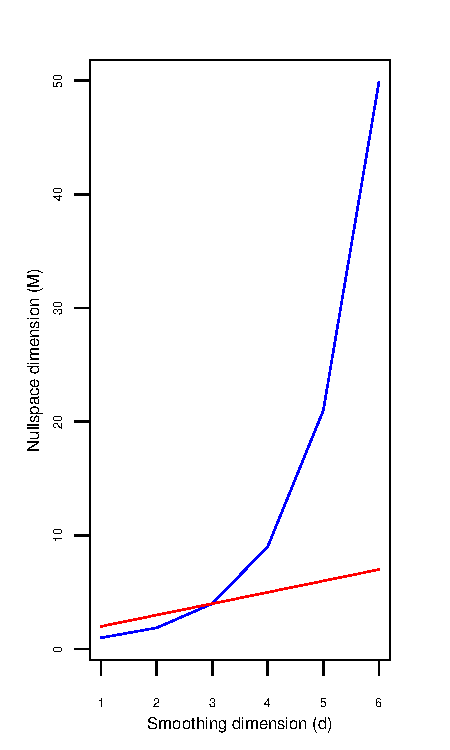
\includegraphics[width=3in]{mds/figs/nullspace-dim.pdf} \\
\caption{Relationship between smoothing dimension ($d$) and the nullspace dimension ($M$) for thin plate regression splines (blue) and Duchon splines (red).}
\label{nullspace-dim}
% generated by thesis/mds/figs/nullspace-dim.R
\end{figure}

\section{Choosing MDS projection dimension}

With Duchon's basis in mind, it is now possible to smooth a space of any dimension using an order 2 penalty, simply by picking $s$ appropriately. Picking the dimension of the MDS projection is now a concern since there is no reason to believe that simply going to higher and higher dimensions will yield better and better results. Keeping in mind the desire for a simple model, it would be preferable to keep the dimension of the projection as small as possible.

\subsection{Using proportion of variation explained}

It is clear that as higher and higher projections are used, a larger and larger proportion of the variation in the distance matrix is explained. It therefore seems reasonable to base the choice of dimension on the proportion of the variation explained in the initial grid. However, what proportion should be used? 80\%? 90\%? 99\%? There is no reason to choose any one of these over the others. Setting the proportion of variation to be explained generally is surely a bad idea, since what works for one domain may well be a disaster for another.


\subsection{Using GCV scores}

Since fitting a GAM with a Duchon spline basis is relatively cheap compared to the cost of finding the within-area distances, the GCV score can be used to find an optimal dimension for the MDS projection. So, using this to our advantage, a series of projections can be tried, their GCV scores calculated, and the best selected as the projection to use for the model.

In particular, starting from a 2-dimensional projection, the dimensionality is increased  and models fitted, until there i an increase in GCV score. The upper bound is the number of dimensions that explain 95\% of the variation in the distance matrix of the initial grid (see section \ref{mds-prac}).  This favours simpler models (in dimensionality terms), although of course a full search can be performed if there is some prior belief that the dimensionality should be higher (indeed there is no reason to believe that the GCV score should be unimodal in dimension). Simulations show that the minima in the GCV score and MSE are in agreement.

Figure \ref{wt2-gcv-projdim-boxplot} shows a plot of GCV score and mean squared error for 60 simulations from the peninsula domain, for each of the 60 realisations a [[new NAME]] was fitted using a 2 through 20 dimensional projection. The boxplots are grouped according to the dimension of the MDS projection used. The graph shows that there is a minima in the score when the dimension is four which corresponds with the minimum MSE.

\begin{figure}
\centering
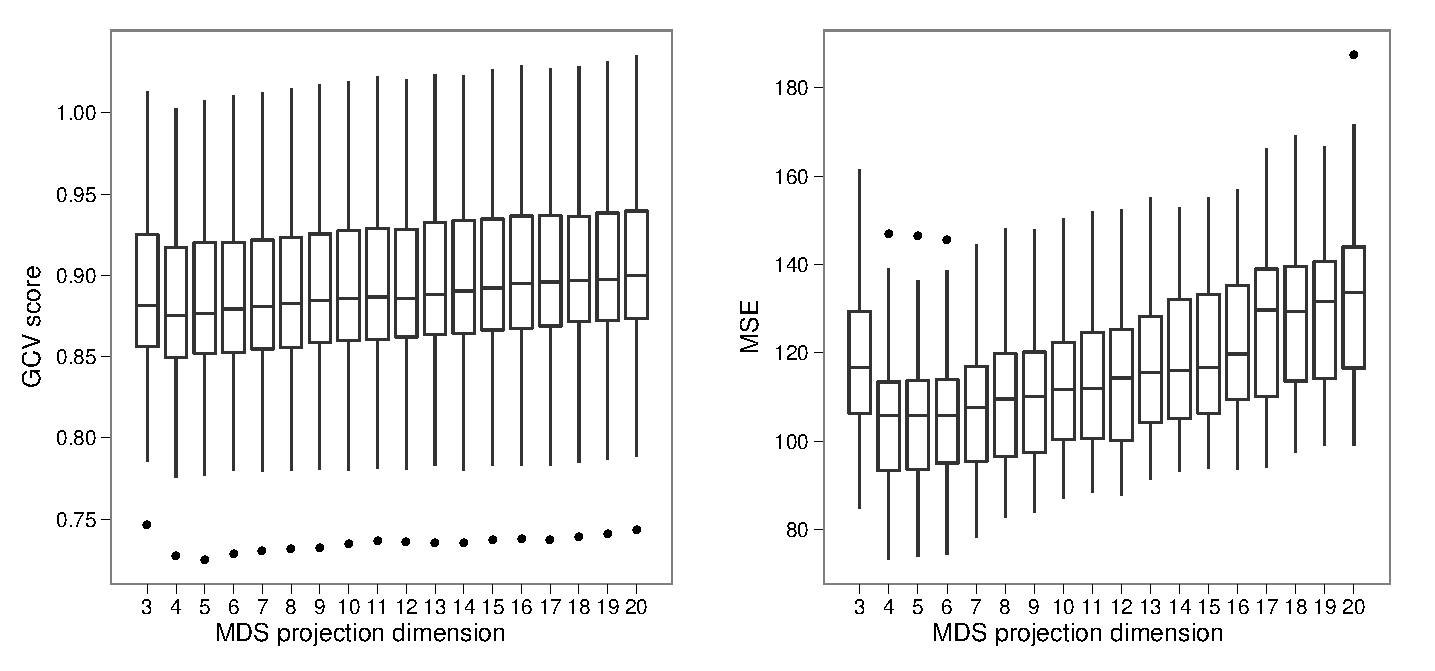
\includegraphics[width=6in]{mds/figs/wt2-gcv-projdim-boxplot.pdf} \\
\caption{MSE and GCV score for the wiggly top domain when different dimensional projections are used. Here a 4-dimensional projection gives a minimum GCV score and MSE.}
\label{wt2-gcv-projdim-boxplot}
% generated by mds/duchon/wt2-gcvml.R
\end{figure}

There is, of course, no guarantee that there will always be a minimum to find and as with all automated methods, practitioners should be mindfull of what could potentially go wrong. However, in the situations tested, this method appeared to be satisfactory.

\section{Within-area distance examples}
\label{gds-wad-examples}
\subsection{Simulations}

Returning to the simulation study in section \ref{wt2bigsim}, the same set of simulations (250 samples at three error levels) was re-run but now using the Duchon splines, selecting MDS dimension based on GCV score (maximum basis dimension was set at 100). The results are shown for the original simulations along side those for the new model (those models which did not to very well originally are excluded).

Figure \ref{wt2-boxplot-duchon} shows the boxplots for these simulations, the [[GIVE THIS A NAME]] method does better than the soap film smoother when the noise is low and was indistinguishable (via a paired Wilcoxon signed rank test) from the soap film smoother at higher noise levels.

\begin{figure}
\centering
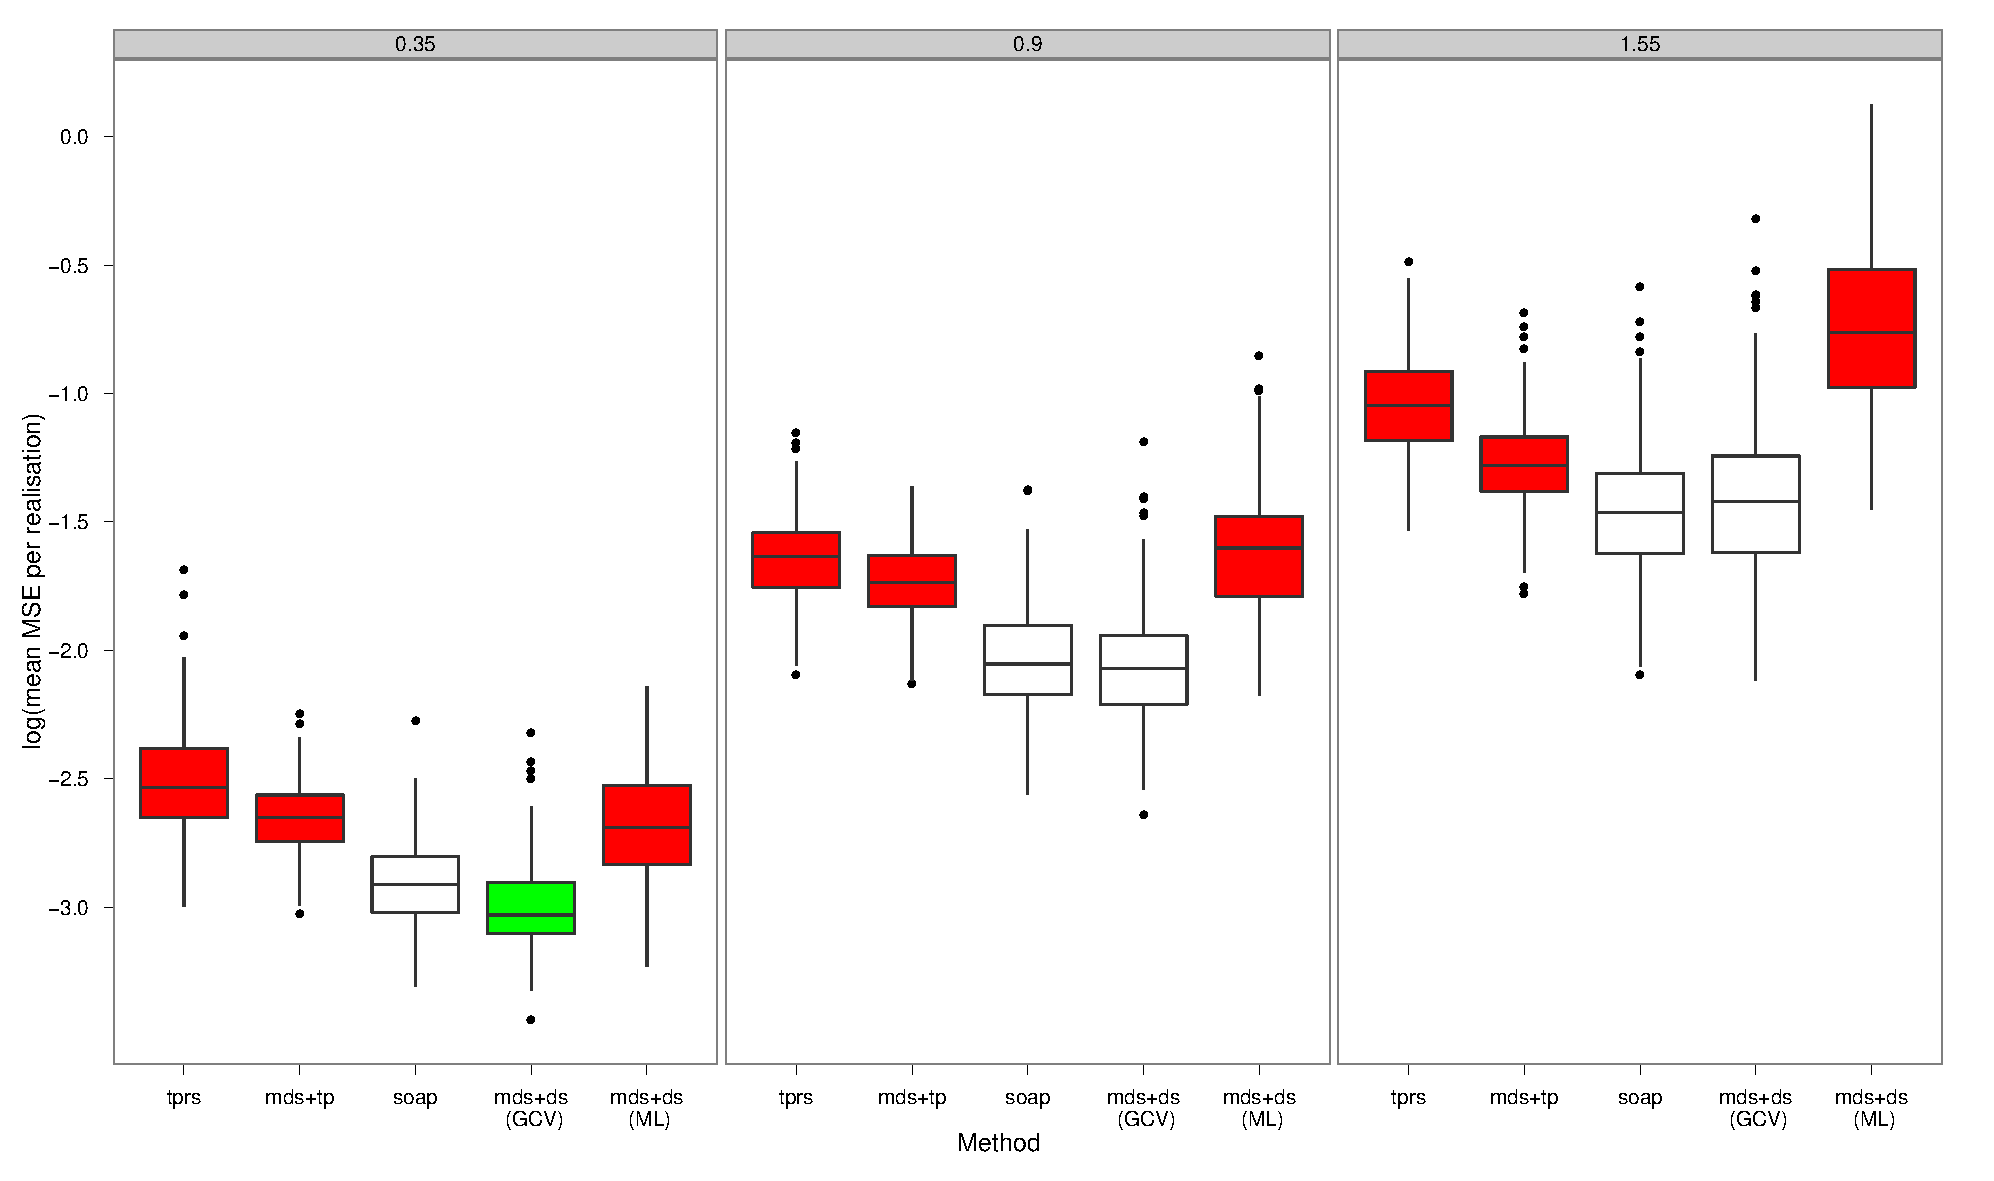
\includegraphics[width=6in]{mds/figs/wt2-boxplot-duchon.pdf} \\
\caption{Boxplots of logarithm of per realisation average mean squared error from simulations on the wiggly top domain. The boxplots are in groups of four for each error level $(\sigma = 0.35, 0.9, 1.55)$. Colours indicate the result of a Wilcoxon paired signed rank test of whether the MSE was significantly (p$<10^{-2}$) different from the soap film smoother. Red indicates different and worse, green different and better.}
\label{wt2-boxplot-duchon}
% generated by mds/duchon/bigsim/boxplot-wt2.R
\end{figure}

[[new wt2??]]

[[aral sim as before?]]

[[ramsay??]]



\subsection{Revisiting the Aral sea}

Going back to the Aral sea example from section \ref{aral-sec}, we can fit a model using the optimal (in a GCV score sense) dimension. Figure \ref{mds-aral-5d-duchon} shows the raw data and a smoothed version, using a 5-dimensional projection (given by minimising the GCV score). The plot does not contain any of the artefacts that were present in the previous smooths of the data.

\begin{figure}
\centering
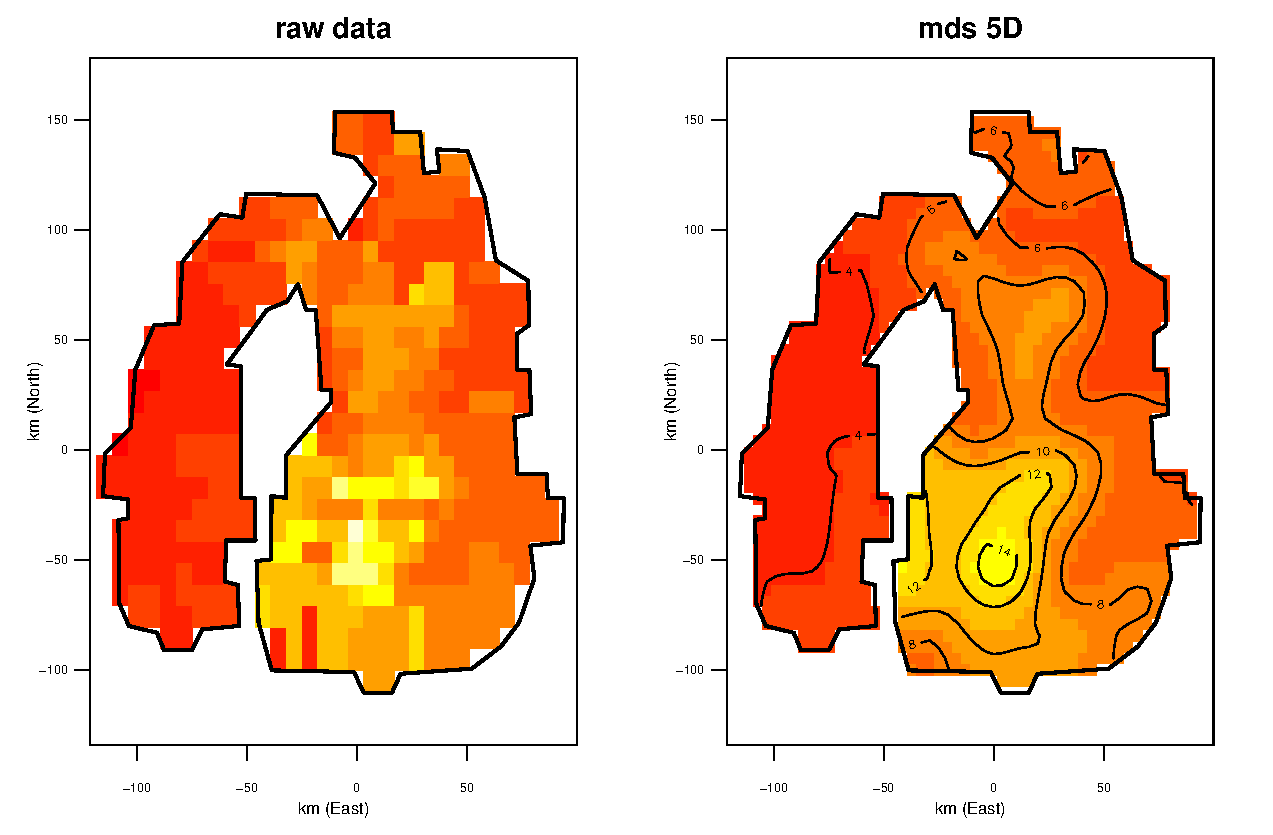
\includegraphics[width=6in]{mds/figs/aral-5d-duchon.pdf} \\
\caption{The Aral sea chlorophyl levels smoothed using Duchon splines, when a 5-dimensional MDS projection is employed. Note the lack of artefacts in comparison to previous \mdsap\ models.}
\label{mds-aral-5d-duchon}
% generated by duchon/aral-evolve.R
\end{figure}



\section{Generalized distance smoothing}
\label{gds-gds-examples}

Duchon splines are able to smooth in high dimensions without the usual problems that come from such situations. Multidimensional scaling allows the projection of any arbitrary distance matrix [TKTKTK check] into Euclidean space. The combination of these two methods has been sucessful in the within-area distance case above, but also allows for smoothing using any set of distances.

Data are often collected on scales that are not necessarily physically meaningful (for example in psychological studies or attitude surveys) but the data are used as if the scale was absolute in some sense. In such cases the distances between the observations may be meaningful but not the actualy ordinal values.

Taking data which is either already distances or distances calculated from data, the MDS projection can be found and then a smooth over those data can be used to model some response.

% concrete example of the above

% measurement error

%
\subsection{Examples}

\textbf{SOME BLURB HERE}


\subsubsection{MP data}




\subsubsection{Breast cancer microarrays}




\subsubsection{Leukemia microarrays}



\section{Software implementation - \mdspack}

The methods detailed in this section, namely the use of Duchon splines along with MDS to perform smoothing are provided in the \textsf{R} package \mdspack\ which is available at A WEBSITE THAT MIGHT BE CRAN.



